\section{Расчет теплового режима РЭС при естественном воздушном охлаждении.}
%% 4.2

Расчет теполового режима радиоэлектронных аппартов рекомендуется
проводить в три этапа~\cite{Rotkop1976}:
\begin{enumerate}[label={\arabic*.}]
  \item Определение среднеповерхностной температуры платы с
расположенными ней деталями, корпуса и температуры воздуха внтури
радиоэлектронного аппарата.
  \item Определить среднеповерхностные температуры корпусов элементов
  используя результаты первого этапа.
  \item Определить максимальные температуры критических зон элементов и
их функциональные связи со среднеповерхностной температурой как
корпусов, так и и плат.
\end{enumerate}

Первый и второй этапы расчета позволяют получить значения основных
параметров, связанных с выбором системы охлаждения, т.е. первых двух
этапов хватает для принятия конструкторсого решения касаемо выбора
системы охлаждения.

Полную систему уравнений теплообмена для реального аппарата часто
невозможно не только решить аналитически, но и строго записать. В
связи с этим процессы, протекающие в реальном радиоэлектронном
аппарате, схематизируют, принимают ряд упрощающик предпосылок и в
результате получают тепловую модель аппарата, для которой и проводят
рассчет теплового режима ~\cite{Rotkop1976}.

Наибольшее распространение получила весьма плодотворная схематичзация
процессов теплообмена в РЭА, предложенная Г.Н.Дульневым
~\cite{Dulnev1968}.

Суть метода заключается в том, что печатная плата с её элементами
принимается за одно тело с изотермической поверхностью (нагретую
зону), для которого и проводится расчет теплового режима.

Таким образом производится расчет среднеповерхностной температуры
нагретой зоны.

Под понятием нагретая зона понимается поверхность того элемента на
печатной плате, который рассеивает больше всего мощности.

В данном случае им является процессор ТNETD 7300.

В указанных ранее источниках нет инфомации о том каков коэффициент
заполнения $K_\mathrm{з}$ для данной РЭС. Однако его можно найти,
опираясь на данные о используемых в РЭС элементах.

Для того чтобы это сделать:
\begin{enumerate}[label={\arabic*.}, nosep]
  \item Найдём объём элементов, опираясь на информацию о чипсете и
принципиальную схему.
  \item Рассчитываем объём корпуса опираясь
    на фото устройства ~\cite{EXTERNAL_PHOTOS}.
  \item По формуле найдём коэффициент заполнения.
\end{enumerate}


Коэффициент запонения вычисляется по формуле ~\cite{Rotkop1976}:
\begin{equation}
  K\mathrm{з} = \sum^n_{i=1} v_{i}/V 
\end{equation}

Здесь $v_i$ – это объём i-того элемента РЭС  $V\mathrm{_э}$, а $V$ – объём
занимаемый корпусом.

Согласно буклету производителя чип ТNETD7300 принадлежит к
вычислительной архитектуре RISC MIPS 32 ~\cite{AR7_fact_sheet}.

Понимание того, к какой архитектуре относится процессор позволяет
определить чипсет, который им используется.

Чипсет, размещаемый на материнской плате, выполняет функцию связующего
компонента (моста), обеспечивающего взаимодействие центрального
процессора (ЦП) c различными типами памяти, устройствами ввода-вывода,
контроллерами, как непосредственно через себя, так и через другие
контроллеры и адаптеры, с помощью многоуровневой системы
шин~\cite{Avdeev2019}.


Без чипсета процессор не сможет взаимодествовать с переферийными
устройствами напрямую.

В свою очередь, данные о
чипсете позволяют сделать вывод о том какова площадь поверхности
элемента.


Исходя из даты изготовления всей РЭС и архитекутры конкретного чипа,
можно сделать вывод, что процессор размещается на чипсете R8000
~\cite{R8000_physical_wikipedia}.

Согласно этим данным чипсет имеет форму прямоугольника со сторонами в
$l_1$ = 17,34 мм и $l_2$ = 17,30 мм (занимает площадь 299,98 мм$^2$) и
рассеивает 13 ват мощности.

Основываясь на информации о процессорах тех лет, примем высоту чипа
$l_3$ равной 2,5 мм ~\cite{MobilePentium3_wikipedia}.

Таким образом можно найти объём элемента пользуясь простой формулой:

\begin{equation}
  V \mathrm{_э} = l_1 \cdot l_3 \cdot l_3
\end{equation}

В данном случае объём элемента равен
$v_1 = 749.955 \mathrm{мм} \approx 750 \mathrm{мм}^3$


Кроме непосредственно процессора для нахождения коэффициента
заполнения разумно также найти объёмы следующих элементов:
\begin{itemize}[nosep]
\item флеш памяти AM29LV160DB;
\item запоминающиго устройство MT48LC;
\end{itemize}

Согласно документации~\cite{FlashMemoryDatasheet} размеры
флеш-памяти
таковы:
длина $l_1$ = 18,40 мм, ширина $l_2$ = 12,00 мм, высота $l_3$ = 1,2 мм.
Таким образом объём элемента $v_2$ равен $264,96 \mathrm{мм}^3$.

Размеры запоминающего устройства приводятся~\cite{SDRAM_Datasheet}
следующие: длина $l_1$ = 22,20 мм, ширина $l_2$ = 11,86 мм, высота
$l_3$ = 1,2 мм. Его объём $v_3$ равен $315,95 \mathrm{мм}^3$

%% Здесь начинается кусок второй главы про размер корпуса
Определим размеры корпуса РЭС использую фотографию его внешнего
устройства. Для этого измерим экранной линейкой величину корпуса,
затем велечину, приложенной для масштаба, рулетки на фотографии и
посчитаем пропорцию.


\begin{figure}[h]
  \centering
  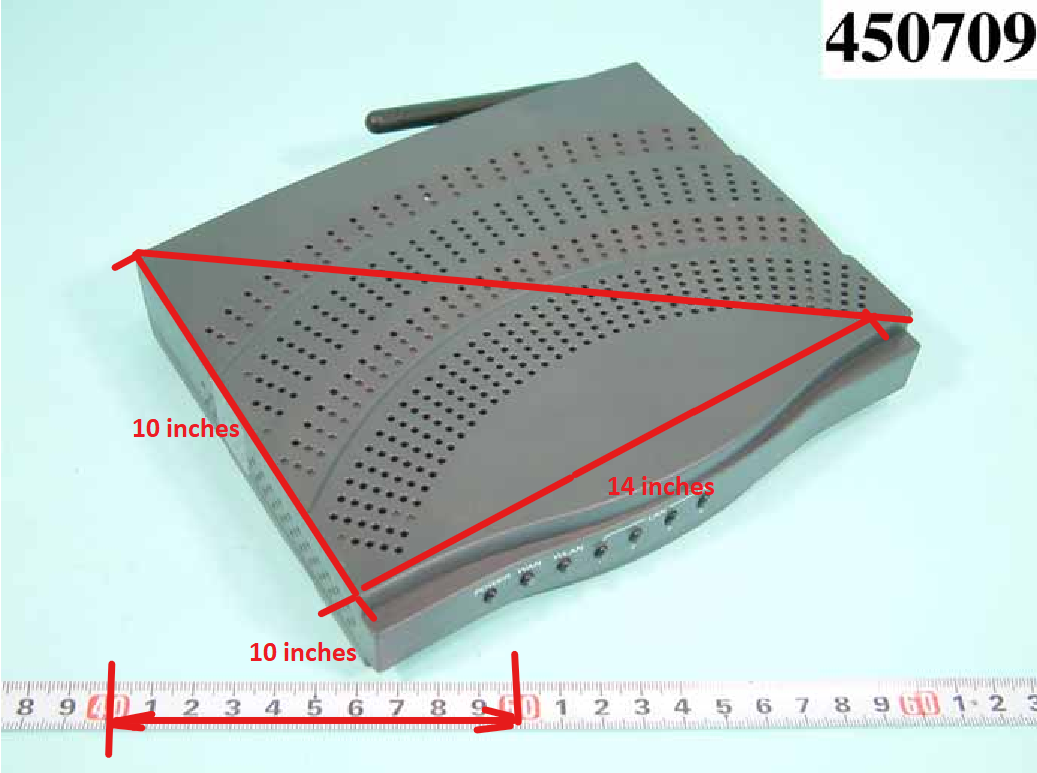
\includegraphics[scale=0.5]{external_photos_size-0.png}
  \caption{Расчет длины и ширины корпуса РЭС, произведенный с помощью
экранной линейки}
\end{figure}



\begin{figure}[h]
  \centering
  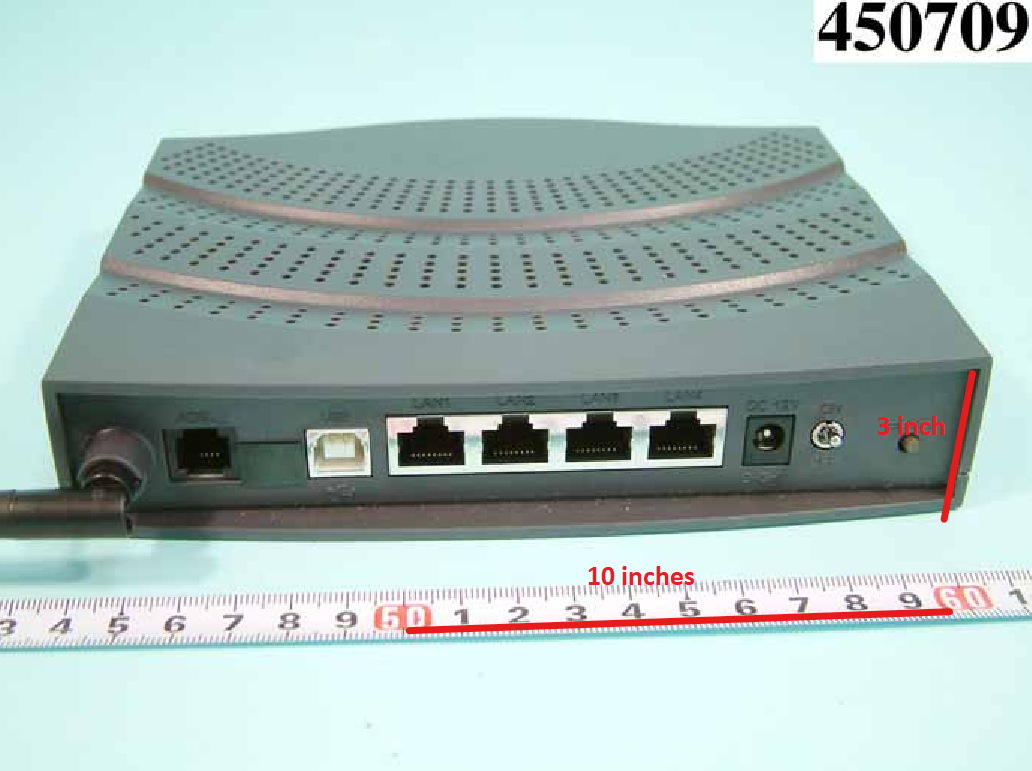
\includegraphics[scale=0.5]{external_photos_size-1.png}
  \caption{Расчет высоты корпуса РЭС, произведенный с помощью
экранной линейки}
\end{figure}
\newpage


\begin{table}
Сконвертируем полученные данные в метрическую систему мер:\\
  \centering
\begin{tabular}[b]{c | c}

    \hline
  Дюймы & Миллиметры \\ 
  10    & 254 \\
    14    & 355,6 \\
  3     & 76,2 \\

\end{tabular}
\end{table}

Таким образом объём корпуса равен:
$$V\mathrm{_К} = 254 \mathrm{мм} \cdot 355,6 \mathrm{мм} \cdot 76,2 \mathrm{мм} = 6882 566,88 \mathrm{мм^3}$$

Рассчитаем коэффициент заполнения как отношения объёма отдельных элементов, к объёму всего корпуса:

$$ K\mathrm{з} = \sum^{n=3}_{i=1} v_{i}/V$$

$$K\mathrm{з} = \frac{264,96 \mathrm{мм}^3 + 315,95 \mathrm{мм}^3 + 750 \mathrm{мм}^3}{6882 566,88 \mathrm{мм^3}} $$

$$K\mathrm{з} = \frac{1 330,9}{6882 566,88}$$

$$K\mathrm{з} \approx 2 \cdot 10^{-4}$$

Найденный коэффициент заполнения, позволит рассчитать условную
поверхность нагретой зоны, по формуле~\cite{Rotkop1976}:
\begin{equation}
  S\mathrm{_з} = 2(l_1 l_2 + (l_1+l_2) l_3 K\mathrm{_з})
\end{equation}

$$S\mathrm{_з} = 0,1805 \mathrm{м^2}$$

По аналогичной формуле находится поверхность корпуса блока:
\begin{equation}
  S\mathrm{_к} = 2(l_1l_2 + (l_1 + l_2)l_3)
\end{equation}

$$S\mathrm{_к} = 1,108\mathrm{м^2}$$

Определяется удельная мощность корпуса блока~\cite{Rotkop1976}:

\begin{equation}
  q\mathrm{_к} = P\mathrm{_з}/S\mathrm{_к}
\end{equation}

$$q\mathrm{_к} = 0,617 \mathrm{ВТ/м^2}$$
\newpage

Рассчитывается удельная мощность нагретой зоны ~\cite{Rotkop1976}:

\begin{equation}
  q\mathrm{_з} = P\mathrm{_з}/S\mathrm{_3}
\end{equation}

$$q\mathrm{_з} = 3,7893 \mathrm{ Вт/м^2}$$

\subsection{Расчет теплового режима РЭС в герметичном корпусе}
%% 4.2.1


\begin{enumerate}[label={\arabic*.}]
\item Найдём коэффициенты
$\vartheta_1$ и $\vartheta_2$ зависящие
от удельной мощности корпуса и удельной мощности нагретой зоны.

\begin{equation}
\vartheta_1 = 0,1472q\mathrm{_к} - 0,2962 \cdot 10^{-3}q\mathrm{_к}^2 + 0,3127 \cdot 10^{-6}q\mathrm{_к}^2
\end{equation}

$$\vartheta_1=0,906$$\\

\begin{equation}
\vartheta_2 = 0,1390q\mathrm{_к} - 0,1223 \cdot 10^{-3}q\mathrm{_к}^2 + 0,0698 \cdot 10^{-6}q\mathrm{_з}^3
\end{equation}

$$\vartheta_2 = 0,525$$


\item Определим перегрев корпуса блока $\vartheta\mathrm{_к}$,
  выбрав коэффициент $K\mathrm{_{Н1}}$ на основании данных из
  ГОСТ~\cite{GOST_15150-69}.

  \begin{equation}
    \vartheta\mathrm{_к} = \vartheta_1 \cdot K\mathrm{_{Н1}}
  \end{equation}

  $K\mathrm{_{Н1}} = 0,999$, $\vartheta\mathrm{_к} = 0,905 K$

\item Рассчитаем перегрев нагретой зоны $\vartheta\mathrm{_з}$,
  выбрав коэффициент $K\mathrm{_{Н2}}$ на основании данных из
  ГОСТ~\cite{GOST_15150-69}.
  \begin{equation}
    \vartheta\mathrm{_з} = \vartheta\mathrm{_к} + (\vartheta_2 - \vartheta_1) \cdot K\mathrm{_{H2}}
    \end{equation}

    $K\mathrm{_{Н2}} = 0,996$, $\vartheta\mathrm{_з} = 0,525 K$

  \item Определим средний перегрев воздуха в корпусе
    \begin{equation}
      \vartheta\mathrm{_в} = 0,5 \cdot (\vartheta\mathrm{_к} + \vartheta\mathrm{_з})
    \end{equation}
    $$\vartheta\mathrm{_в} = 0,0307 К$$

  \item Определим удельную мощность элемента, используя данные о плошади
корпуса
    \begin{equation}
      q\mathrm{_{Эл}} = \frac{P\mathrm{_{Эл}}}{S\mathrm{_{кор}}}
    \end{equation}

    $$S\mathrm{кор} = 0,254\mathrm{м} \cdot 0,354\mathrm{м} = 0,09017\mathrm{м^2}$$
    $$q\mathrm{_{эл}} = \frac{13}{0,09017} =144,172\mathrm{ВТ/м^2} $$

  \item Определим перегрев поверхности элемента.
    \begin{equation}
      \vartheta\mathrm{_{Эл}} = \vartheta\mathrm{_{з}}(a + b \frac{q\mathrm{_{ПП}}}{q\mathrm{_{з}}})
    \end{equation}
    $$\vartheta\mathrm{_{ПП}} = 5,03K$$

  \item Рассчитаем перегрев окружающей элемент среды
    \begin{equation}
      \vartheta\mathrm{_{эс}} = \vartheta\mathrm{_в}(0,75 + 0,25\frac{q\mathrm{_{эл}}}{q\mathrm{_{з}}})
    \end{equation}
    $$\vartheta\mathrm{_{эс}} = 2,95К$$
  \item Определим температуру корпуса блока
    \begin{equation}
      T\mathrm{_к} = \vartheta\mathrm{_к} + T\mathrm{_с}
    \end{equation}
    $$T\mathrm{_к} = 313,019K$$
  \item Определим температуру нагретой зоны
    \begin{equation}
      T\mathrm{_з} = \vartheta\mathrm{_з} + T\mathrm{_c}
    \end{equation}
    $$T\mathrm{_з} = 313,052 K$$

  \item Определим температуру поверхности элемента
    \begin{equation}
      T\mathrm{_{Эл}} = \vartheta\mathrm{_{Эл}} + T\mathrm{_c}
    \end{equation}
    $$T\mathrm{_{Эл}} = 318,030 K$$

  \item Определим среднею температуру воздуха в корпусе
    \begin{equation}
      T\mathrm{_{воз}} = \vartheta\mathrm{_в} + mathrm{_c}
    \end{equation}

    $$T\mathrm{_{воз}} =313,031 K$$
  \item Определим температуру окружающий элемент среды
    \begin{equation}
      T\mathrm{_{эс}} = \vartheta\mathrm{_{эс}} + T\mathrm{_c}
    \end{equation}
    $$T\mathrm{_{эс}} = 315,949 K$$
\end{enumerate}

\subsection{Расчет теплового режима РЭС в герметичном корпусе с внутренним перемешиванием}
%% 4.2.2.

\begin{enumerate}[label={\arabic*.}]
\item Найдём коэффициенты
$\vartheta_1$ и $\vartheta_2$ зависящие
от удельной мощности корпуса и удельной мощности нагретой зоны.

\begin{equation}
\vartheta_1 = 0,1472q\mathrm{_к} - 0,2962 \cdot 10^{-3}q\mathrm{_к}^2 + 0,3127 \cdot 10^{-6}q\mathrm{_к}^2
\end{equation}

$$\vartheta_1=0,906$$\\

\begin{equation}
\vartheta_2 = 0,1390q\mathrm{_к} - 0,1223 \cdot 10^{-3}q\mathrm{_к}^2 + 0,0698 \cdot 10^{-6}q\mathrm{_з}^3
\end{equation}

$$\vartheta_2 = 0,525$$

\item Рассчитаем объём воздуха в корпусе
  \begin{equation}
    V\mathrm{_в} = l_1 l_2 l_3 (1 - K\mathrm{_з})
  \end{equation}

  $$V\mathrm{_в} = 0,687\mathrm{м^3}$$
  \item Поскольку в данном курсвом
    проекте рассмотрено \textbf{естественное} воздушное охлаждение.
    То разумно допустить, что вентилятор в корпусе отсуствует, т. е.
    скорость перемешивания воздуха в корпусе $W$ равно нулю.
    В обратном бы случае охлаждение считалось бы принудительным.

    $$W = 0$$
    
    \item Поскольку скорость перемешивания равна нулю, то зависящей от
      скорости пермешивания коэффицент $K_W$ также равен нулю.
      %% Сюда вставить этот график из matplotlib
    \item Найдем коэффицент $K_W$. Исходя из графика зависимости
коэффициента $K_W$ от скорости перемешивания, можно сделать вывод, что
при нулевой скорости перемешивания, коэффицент равен единице.
$$K_W = 1$$

\item Определим перегрев корпуса блока $\vartheta\mathrm{_к}$,
  выбрав коэффициент $K\mathrm{_{Н1}}$ на основании данных из
  ГОСТ~\cite{GOST_15150-69}.

  \begin{equation}
    \vartheta\mathrm{_к} = \vartheta_1 \cdot K\mathrm{_{Н1}}
  \end{equation}

  $K\mathrm{_{Н1}} = 0,999$, $\vartheta\mathrm{_к} = 0,905 K$

\item 
\item Формула же определения перегрева нагретой зоны отличается от той,
  что была в предыдущем подразделе:
  \begin{equation}
    \vartheta\mathrm{_з} = \vartheta_1(K\mathrm{_{Н1}} - 1) + \vartheta_2
    \end{equation}

    $$\vartheta\mathrm{_з}=0,525$$
  \item Определим средний перегрев воздуха в блоке.
    \begin{equation}
      \vartheta\mathrm{_{вос}} = 0,75 \cdot \vartheta\mathrm{_з}
    \end{equation}
    $$\vartheta\mathrm{_{вoc}} = 0,0393$$
  \item Удельная мощность элемента найдена в предущем подразделе
    $q\mathrm{_{Эл}} =144,172\mathrm{ВТ/м^2} $


      
\end{enumerate}
\subsection{Расчет теплового режима РЭС в герметичном корпусе с наружным обдувом}
%% 4.2.3.

\subsection{Расчет теплового режима РЭС в герметичном оребрённом корпусе}
%% 4.2.4

\subsection{Расчет теплового режима РЭС в перфорированном корпусе}
%% 4.2.5

\subsection{Расчет теплового режима РЭС при принудительном охлаждении}%% 4.2.6